% Trying to break the document up a bit.  This command simply inserts the contents of the file at this point.  It contains the document license, preamble, and title page: things that aren't likely to change more than once.  This can be used to separate discrete parts of a document into files that are easier to edit at one time.
%%%%%%%%%%%%%%%%%%%%%%%%%%%%%%%%%%%%%%%%%%%%%%%%%%%%%%%%%%%%%%%%%%%%%%
% This layout was adapted from one found at latextemplates.com which
% was adapted from another.
%
% License: CC BY-NC-SA 3.0
% (http://creativecommons.org/licenses/by-nc-sa/3.0/)
%
% Original header:
%
% This is a LaTeX version of the sample laboratory report from
% Virginia Tech's copyrighted 08-09 CHEM 1045/1046 lab manual.
% Reproduction of this one appendix section for academic purposes
% should fall under fair use.
%
%%%%%%%%%%%%%%%%%%%%%%%%%%%%%%%%%%%%%%%%%%%%%%%%%%%%%%%%%%%%%%%%%%%%%%

\documentclass{article}

\usepackage{graphicx}
% \usepackage[acronym]{glossaries} % Lets us use acronyms
\usepackage{multicol}
\usepackage{amsmath}
\usepackage{siunitx} % SI units in math mode
%\usepackage[usenames]{color}
\usepackage{subcaption}

\author{}
\title{ELEC-313 \\ Lab 9: Common-Emitter Transistor Amplifier\\ }
\date{\today}

% \loadglsentries{acronyms} % Actually loads 'acronyms.tex'
% \makeglossaries

\begin{document}

\maketitle

\begin{center}
  \begin{tabular}{lr}
    Date Performed: & November 20, 2013 \\
    Partners:       & Charles Pittman    \\
    & Stephen Wilson     \\
  \end{tabular}
\end{center}

\newpage

%\tableofcontents
%\listoffigures
%\listoftables
%\newpage

% Number the enumerate environment (unordered lists) by letter:
% \renewcommand{\labelenumi}{\alph{enumi}.}

\section{Objective}
\label{sec:objective}

The objective is to construct and observe the operation of a CMOS inverter and NAND gate.

\section{Equipment}
\label{sec:equipment}

\begin{itemize}
\item ALD1105 Dual N-channel and P-channel matched pair MOSFET
\item Power supply: HP E3631A
\item Oscilloscope: Agilent 54622D
\item Function generator: HP 33120A
\end{itemize}

 \section{Schematics}
 \label{sec:schematics}

 \begin{figure}[hbtp]
   \centering
   \begin{subfigure}[b]{0.4\textwidth}
     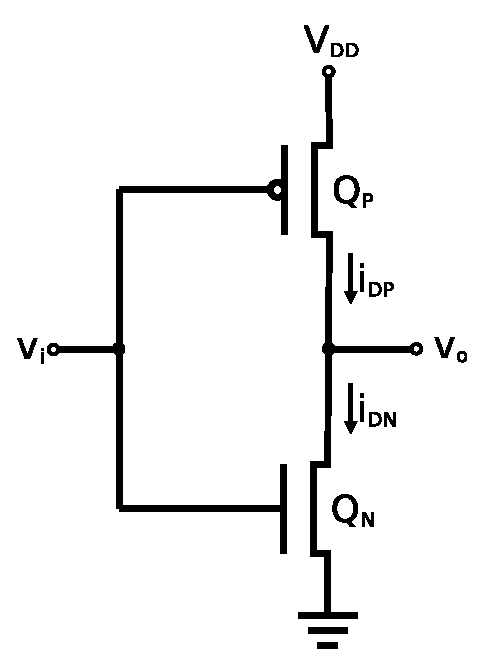
\includegraphics[width=\textwidth]{invert}
     \caption{\label{fig:invert} CMOS Inverter}
   \end{subfigure}%
   ~
   \begin{subfigure}[b]{0.4\textwidth}
     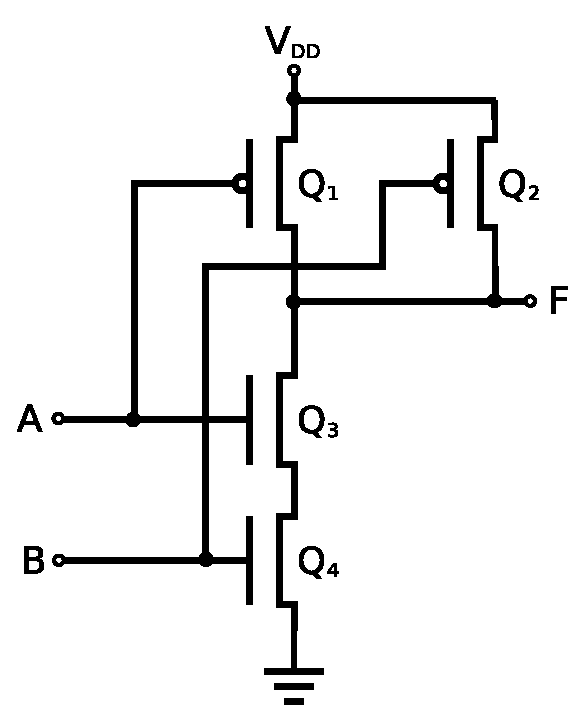
\includegraphics[width=\textwidth]{nand}
     \caption{\label{fig:nand} CMOS NAND}
   \end{subfigure}
   \caption{\label{fig:schematics} Circuits used in this lab.}
 \end{figure}

\section{Procedure}
\label{sec:procedure}

\subsection{CMOS Inverter}
\label{sec:inverter}

% First, the ($+$) and ($-$) terminals of the motor driver board were connected to the \SI{6}{V} DC power supply.  Wires were connected to the motor output terminals on the left side of the motor driver board.  Inputs $L_1$, $L_2$, and $E1-2$ (Enable) were connected in accordance with Table~\ref{tab:logic}.  The output of the DC power supply was set to \SI{6}{V} and the motor output voltage ($V_{out}$) was measured and the LED's were observed, with values recorded in Table~\ref{tab:logic}.  Then, the output of the DC power supply was turned off and \SI{6}{V} DC motor was connected to the output of the motor driver board.  The output of the DC power supply was set to \SI{6}{V} and inputs were connected in accordance with Table~\ref{tab:logic} and the direction of motor rotation was also recorded in Table~\ref{tab:logic}.  Finally, $L_1$, $L_2$, and $Enable$ were set in the clockwise motor rotation and the DC power supply was swept from \SI{6}{V} to \SI{3}{V} in \SI{0.1}{V} increments and the effect on the motor's speed.

\subsection{CMOS NAND}
\label{sec:nand}

% First the function generator was set to a square wave with a frequency of 20 kHz.  Channel 1 of the oscilloscope was connected to the output of the function generator and the square wave was offset for \SI{0}{V} to \SI{5}{V}.  $L_1$ and $L_2$ were again set for clockwise rotation and the $Enable$ input was connected to the function generator.  The DC power supply was turned on and set to \SI{6}{V}.  Then, the \%Duty of the square wave was swept from 20\% to 80\% in 10\% increments and the motor driver board output was recorded in Table~\ref{tab:duty}.  After that, the output of the DC power supply was turned off and the \%Duty of the function generator was rest to 50\%.  Then, the \SI{6}{V} DC motor was connected to the motor output of the motor driver board and the output of the DC power supply was set to \SI{6}{V}.  The \%Duty of the square wave was swept from 50--80\% in 1\% increments and motor speed was observed.

\section{Results}
\label{sec:results}

\begin{figure}[hbtp]
  \centering
  \resizebox{1.0\textwidth}{!}{\input{data1.tex}}
  \caption{\label{fig:data1} Output of CMOS inverter}
\end{figure}

\begin{figure}[hbtp]
  \centering
  \resizebox{1.0\textwidth}{!}{\input{data2.tex}}
  \caption{\label{fig:data2} Data 2}
\end{figure}

\begin{figure}[hbtp]
  \centering
  \resizebox{1.0\textwidth}{!}{\input{data3.tex}}
  \caption{\label{fig:data3} Data 3}
\end{figure}

\begin{figure}[hbtp]
  \centering
  \resizebox{1.0\textwidth}{!}{\input{data4.tex}}
  \caption{\label{fig:data4} Output of CMOS NAND gate}
\end{figure}

% \begin{table}[hbtp]
%   \centering
%   \begin{tabular}{ccc|ccc}
%     Enable & \si{L_1} & \si{L_2} & \si{V_{out}} & LED & Motor \\
%     \hline
%     L & L & L & \SI{-0.01}{V} & off   & off \\
%     L & L & H & \SI{-0.01}{V} & off   & off \\
%     L & H & L & \SI{-0.01}{V} & off   & off \\
%     L & H & H & \SI{-0.01}{V} & off   & off \\
%     H & L & L & \SI{-0.18}{V} & off   & off \\
%     H & L & H & \SI{+5.7}{V}  & red   & CW  \\
%     H & H & L & \SI{+5.5}{V}  & green & CCW \\
%     H & H & H & \SI{+0.01}{V} & both  & off \\
%   \end{tabular}
%   \caption{\label{tab:logic} Logic Table. }
% \end{table}

% \begin{table}[hbtp]
%   \centering
%   \begin{tabular}{cc}
%     Duty Cycle & \si{V_{out}} \\
%     \hline
%     20\% & \SI{-3.01}{V} \\
%     30\% & \SI{-3.39}{V} \\
%     40\% & \SI{-3.76}{V} \\
%     50\% & \SI{-4.13}{V} \\
%     60\% & \SI{-4.49}{V} \\
%     70\% & \SI{-4.84}{V} \\
%     80\% & \SI{-5.19}{V} \\
%   \end{tabular}
%   \caption{\label{tab:duty} Pulse-width modulation}
% \end{table}

\section{Conclusion}
\label{sec:conclusion}

% The motor driver board can be adjusted to control the speed and direction of the DC motor.  First, the $Enable$ input must ``see'' ~\SI{5}{V} before the motor driver board can then allow the $L_1$ and $L_2$ inputs control the phase/rotation of the output.  To control the output rotation, the $L_1$ and $L_2$ inputs must also see ~\SI{5}{V} separately.  In our configuration, $L_1$ caused the motor to rotate counter-clockwise.  Similarly, $L_2$ caused clockwise rotation, so enabling both causes the motor to stop.

% The motor driver board speed was adjusted via two different approaches in the experiment: in part one, the input voltage was adjusted, changing the output voltage;  in part two, the frequency of the input signal was adjusted, which also affected output voltage.

% \section{Equations}
% \label{sec:equations}

% % LaTeX sees blank lines as a start of another paragraph.  To avoid
% % unnecessary vertical spaces between equations, and still visually
% % separate in source, put a comment between them.
% %
% \begin{equation}
%   \label{eq:percent_diff}
%   \%_{diff} = \frac{|nominal - measured|}{nominal}\times 100\%
% \end{equation}
% %
% \begin{equation}
%   \label{eq:ripple}
%   V_r = V_{max} - V_{min}
% \end{equation}
% %
% \begin{equation}
%   \label{eq:volt_reg}
%   \%_{reg} = \frac{V_{load} - V_{no load}}{V_{no load}}\times 100\%
% \end{equation}

\end{document}
